\documentclass{article}
 \usepackage[utf8]{inputenc}
 \usepackage{graphicx}
 \graphicspath{ {images/} }
 \begin{document}

 \title{ARTIFICIAL INTELLIGENCE EXAM}
 \author{Course Code: 1DL340}
 \date{Ref.  This is a student generated exam. }
 \maketitle

 This exam has  6  questions for a total of  19  marks. Grade boundaries are:

 \begin{center}
 3 -  9.5 

 4 -  12.5 

 5 -  15.5 

 \end{center}

 In exceptional circumstances these boundaries may be adjusted at the discretion of the examiner. This would be done on an exam-wide basis, NOT for individual students.

 You are permitted to make use of a calculator and language dictionary in this exam.
\clearpage
\section{MCMC and Directed Graphical Models}

Tables~\ref{MCMC1} to~\ref{MCMC5} provide the conditional probability distributions for a directed graphical model.

A. Use this information to draw the graph of the associated directed graphical model. (1 mark)

B. Table~\ref{MCMC6} provides observed values for some of the nodes. Given these, the initial values provided in Table~\ref{MCMC7} and the random numbers provided below, use the Metropolis within Gibbs MCMC sampling algorithm to generate two complete samples of the variables. Assume that the candidate function gives the opposite of the current value. At each step, explain what value you are considering, what the current and candidate values are, and why you updated it or did not update it. (4 marks)

Random numbers: 0.253,0.603,0.397,0.553,0.698,0.573 
\begin{table}[h!]
\caption{P(A)}
\label{MCMC1}
\begin{center}
\begin{tabular}{ |c||c|c| } 
\hline
 - & A=F & A=T\\
\hline
 & 0.65 & 0.35\\
\hline
\end{tabular}
\end{center}
\end{table}
\begin{table}[h!]
\caption{P(B$|$A)}
\label{MCMC2}
\begin{center}
\begin{tabular}{ |c||c|c| } 
\hline
 A & B=F & B=T\\
\hline
 A=F & 0.3 & 0.7\\
 A=T & 0.15 & 0.85\\
\hline
\end{tabular}
\end{center}
\end{table}
\begin{table}[h!]
\caption{P(C$|$A)}
\label{MCMC3}
\begin{center}
\begin{tabular}{ |c||c|c| } 
\hline
 A & C=F & C=T\\
\hline
 A=F & 0.85 & 0.15\\
 A=T & 0.4 & 0.6\\
\hline
\end{tabular}
\end{center}
\end{table}
\begin{table}[h!]
\caption{P(D$|$B,C)}
\label{MCMC4}
\begin{center}
\begin{tabular}{ |c|c||c|c| } 
\hline
 B & C & D=F & D=T\\
\hline
 B=F & C=F & 0.2 & 0.8\\
 B=F & C=T & 0.6 & 0.4\\
 B=T & C=F & 0.55 & 0.45\\
 B=T & C=T & 0.05 & 0.95\\
\hline
\end{tabular}
\end{center}
\end{table}
\begin{table}[h!]
\caption{P(E$|$C)}
\label{MCMC5}
\begin{center}
\begin{tabular}{ |c||c|c| } 
\hline
 C & E=F & E=T\\
\hline
 C=F & 0.75 & 0.25\\
 C=T & 0.05 & 0.95\\
\hline
\end{tabular}
\end{center}
\end{table}
\begin{table}[h!]
\caption{Observed Values}
\label{MCMC6}
\begin{center}
\begin{tabular}{ |c|c| } 
\hline
 Node & Value \\
\hline
B & FALSE\\
E & FALSE\\
\hline
\end{tabular}
\end{center}
\end{table}
\begin{table}[h!]
\caption{Initial Values}
\label{MCMC7}
\begin{center}
\begin{tabular}{ |c|c| } 
\hline
 Node  & Value \\
\hline
A & TRUE\\
C & TRUE\\
D & TRUE\\
\hline
\end{tabular}
\end{center}
\end{table}
\clearpage
\section{Hidden Markov Models: Forward-Backward Algorithm}

Tables~\ref{hmmfb1} to~\ref{hmmfb4} provide the transition matrix, emission matrix, initial state and a sequence of observations for a hidden Markov model. Use the forward-backward algorithm to calculate the probability distributions for the state of the system at times 0, 1 and 2 given the observations. Show all working. (4 marks)

\begin{table}[h!]
\caption{Transition Matrix}
\label{hmmfb1}
\begin{center}
\begin{tabular}{ |c||c|c| } 
\hline
 $S_{t-1}$ & $S_t$=0 & $S_t$=1\\
\hline
 0 & 0.4 & 0.6\\
 1 & 0.1 & 0.9\\
\hline
\end{tabular}
\end{center}
\end{table}
\begin{table}[h!]
\caption{Emission Matrix}
\label{hmmfb2}
\begin{center}
\begin{tabular}{ |c||c|c| } 
\hline
 $S$ & $E=0$ & $E=1$\\
\hline
 0 & 0.7 & 0.3\\
 1 & 0.7 & 0.3\\
\hline
\end{tabular}
\end{center}
\end{table}
\begin{table}[h!]
\caption{Initial State}
\label{hmmfb3}
\begin{center}
\begin{tabular}{ |c|c| } 
\hline
 $S=0$ & $S=1$\\
\hline
0.5 & 0.5\\
\hline
\end{tabular}
\end{center}
\end{table}
\begin{table}[h!]
\caption{Observations}
\label{hmmfb4}
\begin{center}
\begin{tabular}{ |c|c| } 
\hline
 Time=1 & Time=2\\
\hline
TRUE & TRUE\\
\hline
\end{tabular}
\end{center}
\end{table}
\clearpage
\section{Scheduling}

Provide a complete resource constrained schedule for the actions found in Table~\ref{schActions}. (4 marks)
\begin{table}[h!]
\caption{Actions}
\label{schActions}
\begin{center}
\begin{tabular}{ |c|c|c|c|c|c| } 
\hline
 Index & Action & Duration & Uses & Consumes & After \\
\hline
1 & Start & 0 &   & 0 nails & NA\\
2 & Action 1 & 45 &   & -1 nail & 1\\
3 & Action 2 & 20 &   & 0 nails & 1\\
4 & Action 3 & 35 &  Saw & -1 nail & 1\\
5 & Action 4 & 45 &  Hammer,Saw & 1 nail & 3,2,4\\
6 & Action 5 & 10 &   & 0 nails & 3,5,2\\
7 & Action 6 & 45 &  Hammer,Saw & 0 nails & 6\\
8 & Action 7 & 10 &  Hammer & 1 nail & 7,2,4\\
9 & Finish & 0 &   & 0 nails & 8\\
\hline
\end{tabular}
\end{center}
\end{table}
\clearpage
\section{Basic Feed-Forward ANNs}

Examine the neural network given in the diagram labelled 'Basic Regression Feed-Forward Neural Network'. In this diagram, square nodes represent biases, blue nodes the input layer, green nodes a hidden layer, and red nodes the output layer. The first round blue input node is associated with feature X1, and the second with feature X2 (counting downwards). Assuming that all activation functions are rectifiers (i.e. the hidden nodes are ReLU units), and the output is a basic linear regression function, calculate the output of this network if it was given an input of X1 = -1 and X2 = 4. Show all working. (2 Marks)

\begin{figure}[h!]
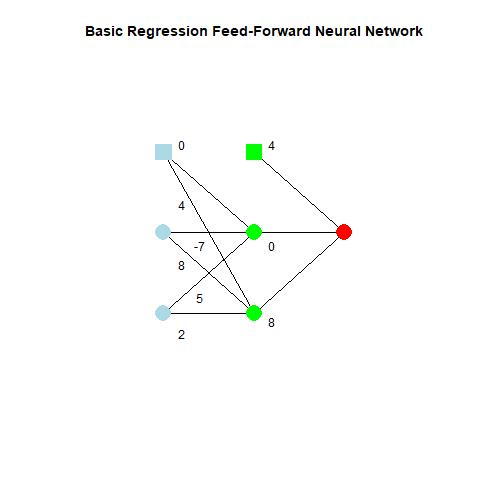
\includegraphics[width=\textwidth]{ffnn.jpg}
\end{figure}
\clearpage
\section{ Planning Graphs }

Explain the two ways a planning graph can be used to provide a heuristic for A*. (2 marks)
\clearpage
\section{ GANs }

Assume you have a GAN where the discriminator network is a simple binary (Genuine/Fake) classifier. Briefly explain how the generator network is trained. (2 marks)

\end{document}
